%%%Slides
\begin{figure}[!ht] \centering  % [h!]
	\caption{Simulated trends from a SIR model of stock investors}
	\label{fig:sir_simulate}
	\centerline{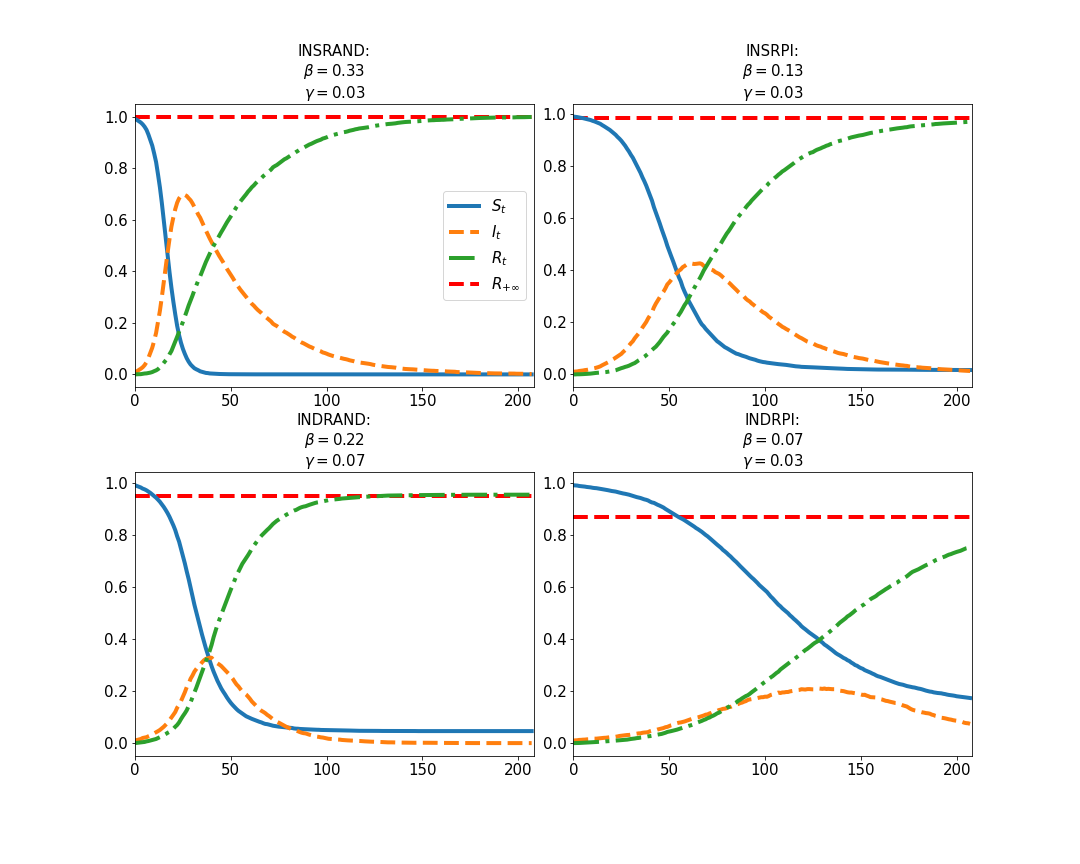
\includegraphics[width=\textwidth]{./figures/sir_simulate.png}}
	\begin{flushleft}
	{\footnotesize Note: this graph plots the simulated paths of populations in different compartments in a SIR model of stock investors, as described in \cite{shiller1989survey}. We use the median estimates of the infection rate $\beta$ and recovery rate $\gamma$ for four samples: institutional investors for a randomly selected stock (INSRAND), institutional investors for a rapidly rising stock (INSRPI), individual investors for a random stock (INDRAND), and individual investors for a rapidly rising stock (INDRPI). The horizontal dashed line corresponds to the limiting size of compartment of $R$ in the long run. The simulation is done with the Python library ``NDlib'', for details, see the companion \href{https://github.com/iworld1991/EpiExp/blob/master/Python/SIR_Ndlib.ipynb}{Jupyter Notebook}. }
				\end{flushleft}
\end{figure}
